%Chapter "Computational aspects"
%
\graphicspath{ {./img/Computational/} }
\chapter{Computational aspects}
\label{chap: Computational Aspects}
\section{Global assembly}
In this section we will discuss the fundamental process of building the system of algebraic equations through the addition or assembly of elemental coefficient matrices as described by \cref{eq:assem} where $K^G$ is the global coefficient matrix; $k^i$ is the local elemental matrix for the $i$-th element; $\assem_{i=1}^{Numel}$ is the assembly operator and $i$ is an element index ranging between $1$ and the total number of elements $Numel$ that conform the finite element model. Notice that the assembly operator is analogous to the sum operator commonly used in the representation of a series of $N$ terms but it contains information indicating the position of each single term from the element coefficient matrix within the global system.
\begin{equation}\label{eq:assem}
{K^G}=\assem_{i=1}^{Numel} k^i.
\end{equation}

In this section we will describe the fundamental algorithmic steps to perform that process. We first summarize the basic general steps and then illustrate the process through a simple example involving a $2D$ mesh of 4-noded elements. The section is complemented with the Python scripts {\bf GLOBAL.py} and the secondary module {\bf assemutil.py}.

\subsection*{The assembly algorithm}
The process of assembly of the elemental coefficient matrices into the global system involves (i) the identification of the active degrees of freedom (or equation numbers) assigned to each node in the mesh (ii) the identification of the relationship between the elemental degrees of freedom and the global degrees of freedom and (iii) the computation of the coefficient matrix for each element in the model.

The first step is easily accomplished by assigning a boundary condition flag to the degrees of freedom existing at each node. Here we use a $0$ value to indicate an active degree of freedom and a $-1$ to indicate a prescribed degree of freedom. This information is stored in a boundary condition array $IBC$, of dimension $nn \times MDIM$, where $nn$ corresponds to the  total number of nodal points and $MDIM$ represents the problem dimensionality. The $IBC$ array is first input by the user and later modified by the program in a process where the boundary condition flag is read and equations are counted and assigned according to the result. If the boundary condition flag is equal to $0$ the program assigns an equation number while it produces a $0$ value if the flag is equal to $-1$.

In the second step the nodes conforming each element are stored in a connectivity array  $IELCON$ of dimension $Numel \times MxNNel$ where $Numel$ is the number of elements in the model and $MxNNel$ is the maximum number of nodes in a given element. Thus each row in the $IELCON$ array stores the nodal point data for the element. Each entry in the $IELCON$ array can now be directly translated into equation numbers using the processed $IBC$ array. This results in the discrete version of the assembly operator $\assem_{i=1}^{Numel}$ also called the assembly list or the $DME$ operator in our codes.

In the final step the mesh is covered one element at a time and each elemental coefficient matrix is assembled into the global matrix as indicated by the $DME$ operator. The actual computation of the elemental matrix is conducted by an element based subroutine, called here $UEL$, which may be different for each element in the mesh according to different kinematic o material assumptions. The complete process is summarized in \cref{algo:overall} where we describe for completeness additional steps involved in the finite element algorithm. We have introduced additional global and elemental arrays $RHS^G$ and $rhs^i$ respectively, storing the element nodal excitation and the resulting vector of global excitation. This vector is assembled simultaneously, and using the same data, with the global coefficient matrix. In the final step in the finite element algorithm the system of equations is solved. Notice that the essential boundary conditions were already considered during the assembly process and as a result the global algebraic system of equations is ready to be solved. Finally, after the system has been properly solved the nodal results are scattered through the elements in a process which is inverse to the assembly operation but that uses the same information contained in the $DME$ operator.

\begin{algorithm}[H]\label{algo:overall}
\SetAlgoLined
\KwData{Finite element model}
\KwResult{Field function}
\BlankLine
READ $IBC$ and $IELCON$ arrays ;\\
Compute modified $IBC$ array ;\\
Compute $DME$ operator (using $IBC$ and $IELCON$ arrays);\\
$K^G \leftarrow 0.0$;\\
\BlankLine
\For{$i \leftarrow 1$ to $Numel$}{
    Call UEL(element parameters;$K^i$) ;\\
    $K^G \leftarrow K^G+K^i$ (Assemble each $k^i$ into $K^G$ according to the $DME$ operator);\\
    $RHS^G \leftarrow RHS^G+rhs^i$ (Assemble each $rhs^i$ into $RHS^G$);\\	
	\BlankLine
	}
\BlankLine
Solve ${K^G}{U^G} = RH{S^G}$;\\
Scatter solution to the elements
\caption{Summarized algorithm for the finite element method}
\end{algorithm}
\newpage

\subsection*{Sample problem}
Consider the mesh shown in \cref{fig:quad}. The problem parameters in this case are $nn=9$, $Numel=4$ and $MxNNel=4$.

\begin{figure}[h]\label{fig:quad}
\centering
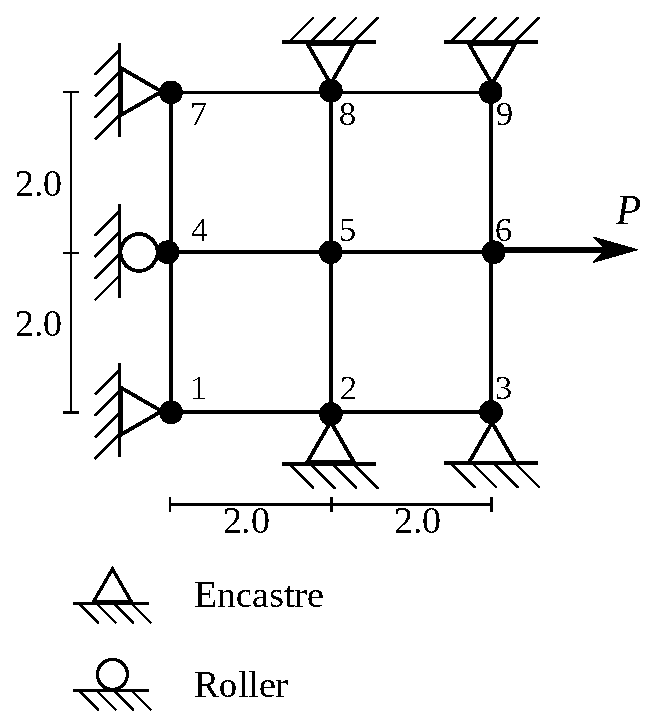
\includegraphics[width=10cm]{mesh2.pdf}
\caption{Finite element mesh of 4-noded elements. The global matrix can be assembled using the python scripts {\bf GLOBAL.py} and the secondary module {\bf assemutil.py}. The input files required to run the script are called {\bf nodes.txt} and {\bf eles.txt}}
\end{figure}



The array of boundary conditions as input from the user corresponds to
\[IBC = \begin{bmatrix}
-1 & -1\\
-1 & -1\\
-1 & -1\\
-1 & 0\\
0 & 0\\
0 & 0\\
-1 & -1\\
-1 & -1\\
-1 & -1
\end{bmatrix}\]

while its code-modified version reads
\[IBC = \begin{bmatrix}
0 & 0\\
0 & 0\\
0 & 0\\
0 & 1\\
2 & 3\\
4 & 5\\
0 & 0\\
0 & 0\\
0 & 0
\end{bmatrix}\]

Notice that the program changes each $-1$ entry to a $0$ valued entry and assigns an equation number to the position containing an original $0$ entry during an equation-assigning and equation-counting operation. Similarly, the element connectivity for the current example read
\[IELCON = \begin{bmatrix}
1 &2 &5 &4\\
2 &3 &6 &5\\
4 &5 &8 &7\\
5 &6 &9 &8
\end{bmatrix}\]

The so-called $DME$ operator is actually the same $IELCON$ but translated into equation numbers for each element. Accordingly in the current example we have
\[DME = \begin{bmatrix}
0 &0 &0 &0 &2 &3 &0 &1\\
0 &0 &0 &0 &4 &5 &2 &3\\
0 &1 &2 &3 &0 &0 &0 &0\\
2 &3 &4 &5 &0 &0 &0 &0
\end{bmatrix}\]

The definition of the element connectivity and its subsequent translation into degrees of freedom is carried out according to a local element definition like the one shown in \cref{fig:locdof}

\begin{figure}[H]\label{fig:locdof}
\centering
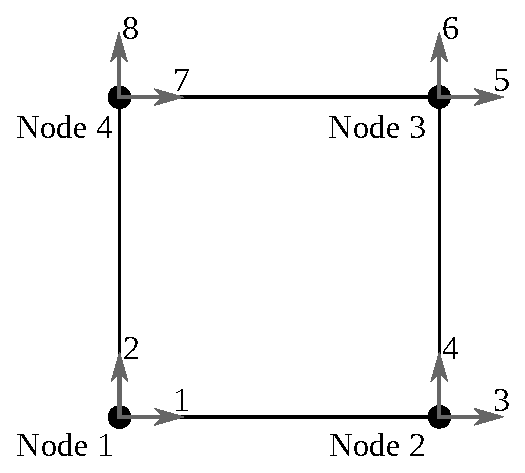
\includegraphics[width=8cm]{localdof.pdf}
\caption{Local definition for a 4-noded element.}
\end{figure}

As a result the $(i,j)$ entry in the $DME$ corresponds to the global equation number associated with the local degree of freedom $j$ of the $i$ element. For instance the value of $4$ stored at position $(2,5)$ in the current $DME$ indicates that the global equation $4$ corresponds to the local equation $5$ (column index) in element $2$ (row index).

The assembly process is then conducted by identifying the relation between the entries in each row of the $DME$ operator and the list of local degrees of freedom for the reference element shown in \cref{fig:locdof}. Accordingly, for element 2 it follows that the assembly of row $5$ of the local stiffness matrix proceeds as follows
\begin{align*}
K_{4,4}^G & \leftarrow  K_{4,4}^G + k_{5,5}^2 \\
K_{4,5}^G & \leftarrow  K_{4,5}^G + k_{5,6}^2 \\
K_{4,3}^G & \leftarrow  K_{4,3}^G + k_{5,8}^2
\end{align*}

In \cref{algo:overall} it must be noticed that the local stiffness matrix for each $i$ element is obtained by the call to the local element subroutine $UEL$. In the script GLOBAL.py these elemental routines produce a fictitious matrix filled out with ones and the actual computation of the elemental coefficient matrix is discussed later.


\section{Sparse assembly}
In Finite Elements is common to have stiffness and mass matrices that are sparse, i.e., matrices in which most of the elements are zero.


For instance, in a regular mesh formed with bilinear quadrilaterals the number of nonzero entries is given by the expression
\[\text{storage} = 9 n_x n_y - 9 n_x - 3 n_y + 4\, ,\]
where $n_x$ is the number of nodes in the $x$ coordinate and $n_y$ is the number of nodes in the $y$ coordinate. Figure \ref{fig:sparse_storage} presents the needed storage for a mesh with $n_x=n_y$ for different sizes.
\begin{figure}[H]
\centering
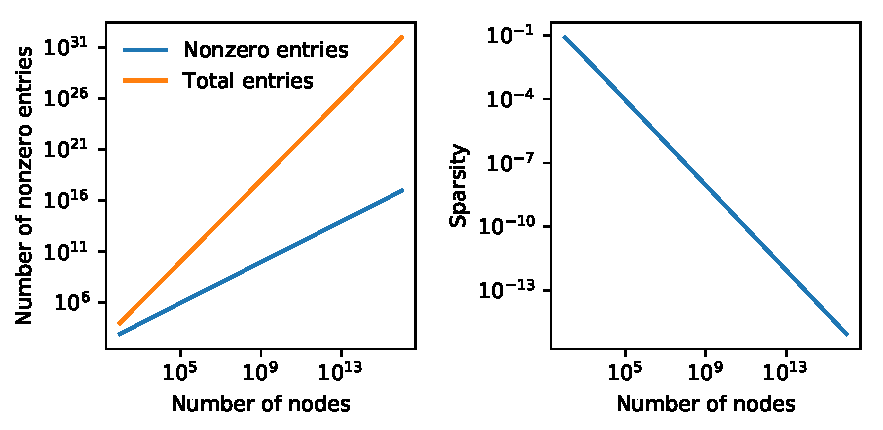
\includegraphics[width=6 in]{sparse_storage.pdf}
\caption{Nonzero entries in a sparse matrix for a structured mesh of bilinear elements.}
\label{fig:sparse_storage}
\end{figure}

\section{Python implementations}


\section{Commercial codes and user subroutines}





